\section{Motivation}
While the output from Grad-CAM does not provide a good insight into what the segmentation neural network is doing, the RISE output is quite usable. When evaluation an interpretability method, not only the method itself but also the trained neural network is analyzed. It is therefore possible that a good method returns bad results because the neural network is of low quality. We therefore decided to generate an artificial dataset (a "toy" example) where there is no doubt about the quality of the trained model.


\section{Introduction}
\nblink{brats/08\_testnet\_generate.ipynb}
\nblink{brats/09\_testnet\_train.ipynb}

The basic idea in this dataset is to show that not only the pixel data inside the segmentation region is relevant for the network, but also other parts of the image. To show this, we built a dataset where one part of the image is essential to generate a correct segmentation output, but itself is not contained in the segmentation output.

2D shapes (circle, square, cross and triangle) are drawn (with the Python Imaging Library) onto images. On the left side of an image, there is always a cross and a triangle displayed. On the right side, in 50\% of the cases a circle is drawn, in the other 50\% a square is drawn. Depending on the shape on the right side (circle or square), one of the shapes on the left side are segmented. If the right shape is a circle, the triangle is segmented. If the right shape is a square, the cross is segmented

\begin{figure}[H]
    \centering
    \begin{subfigure}[t]{.5\textwidth}
        \centering
        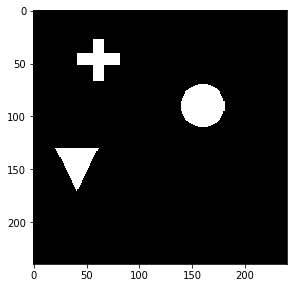
\includegraphics[width=\linewidth]{chapters/05_testnet/images/testnet_a-0.png}
        \caption{Input image}
    \end{subfigure}%
    \begin{subfigure}[t]{.5\textwidth}
        \centering
        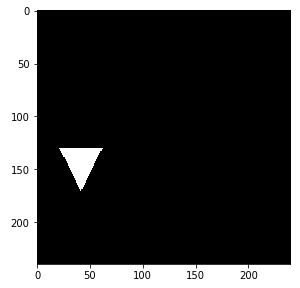
\includegraphics[width=\linewidth]{chapters/05_testnet/images/testnet_a-1.png}
        \caption{The expected output segment}
    \end{subfigure}
    \caption{Testnet with circle: The input image contains a circle on the right, therefore the triangle should be segmented}
    \label{testnet_example_1}
\end{figure}

\begin{figure}[H]
    \centering
    \begin{subfigure}[t]{.5\textwidth}
        \centering
        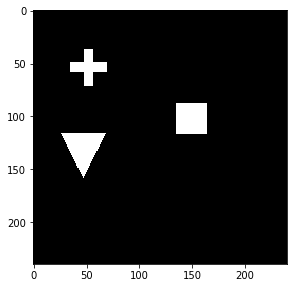
\includegraphics[width=\linewidth]{chapters/05_testnet/images/testnet_b-0.png}
        \caption{Input image}
    \end{subfigure}%
    \begin{subfigure}[t]{.5\textwidth}
        \centering
        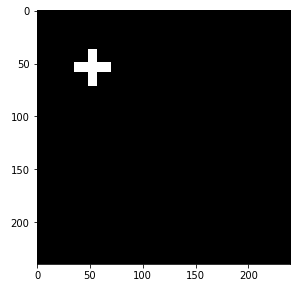
\includegraphics[width=\linewidth]{chapters/05_testnet/images/testnet_b-1.png}
        \caption{Output segment}
    \end{subfigure}
    \caption{Testnet with cube: The input image contains a square on the right, therefore the cross should be segmented}
    \label{testnet_example_2}
\end{figure}

In Figure \ref{testnet_example_1}, the right shape is a circle. Therefore the triangle is segmented in the output.
In Figure \ref{testnet_example_2}, the right shape is a square. Therefore the cross is segmented in the output.

A good interpretability method should not only show an importance on the segment output (circle and cross), but also on the shapes on the right (circle, cross).

\section{Applying RISE}
\nblink{brats/10a\_testnet\_rise\_multipixel.ipynb}

Applying RISE on this dataset is much the same as on the BraTS dataset, the only difference is that BraTS has four channels (one for each modality) and this dataset only has one (grayscale).

\subsection{Results}
\begin{figure}[H]
    \centering
    \begin{subfigure}[t]{.5\textwidth}
        \centering
        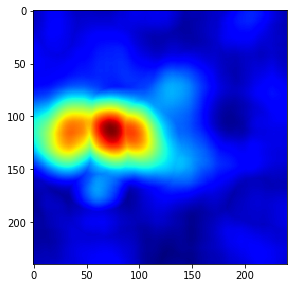
\includegraphics[width=\linewidth]{chapters/05_testnet/images/rise_1-0.png}
        \caption{Saliency map generated using the mean function.}
    \end{subfigure}%
    \begin{subfigure}[t]{.5\textwidth}
        \centering
        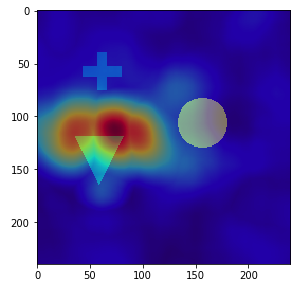
\includegraphics[width=\linewidth]{chapters/05_testnet/images/rise_1-1.png}
        \caption{Saliency map generated using the mean function overlaid on the network input image.}
    \end{subfigure}
    \caption{The saliency map generated by RISE on an sample image of the testnet dataset.}
    \label{testnet_rise_mean}
\end{figure}

\subsection{Discussion}
Figure \ref{testnet_rise_mean} show the saliency map generated by our RISE multi pixel method. We expected from the method that it now only marks the region with the actual segment output (the triangle), but also the circle on the right, because it is essential to generate a correct segmentation output. This method completly missed the importance of the circle.

\subsection{Conclusion}
Sadly, this test dataset confirms that not the neural network but our RISE interpretability method is not good enough to generate results with deep insights into the analyzed model. Not only are the generated saliency maps of low resolution, they also miss an important part of the image (the right side with the circle or square).

We suspect that the masks RISE applies on the input images remove too much information from the image for a segmentation model. Building a method that does the opposite - only removing a small part of the image and then checking if and how much the segmentation did change - is therefore the next obvious step to take.
